\documentclass{beamer}
%\documentclass[handout]{beamer}
\usepackage{graphicx}
\usepackage{amsmath}
\usepackage{amssymb}
\usepackage{amsthm}
\usepackage{array}
\usepackage{xspace}
\usepackage{listings}
\usepackage{todonotes}

\usepackage{bibspacing} 
\usepackage{natbib} 
\bibliographystyle{apalike}

\usepackage{lstjanus}

\newcommand{\basetop}[1]{\vtop{\vskip-1ex\hbox{#1}}}
\newcommand{\source}[1]{\let\thefootnote\relax\footnotetext{\scriptsize\textcolor{kugray1}{Source: #1}}}

\mode<presentation>
{
  \usetheme{Diku}
  \beamertemplatenavigationsymbolsempty
  \setbeamercovered{invisible}
%  \setbeamercovered{transparent}
}


\title[]{Lightweight Crypto in Reverse}
%\subtitle{Unofficial}

\author{Dominik T\'{a}borsk\'{y}\\\texttt{dominik.taborsky@protonmail.ch}}
%\institute{DIKU\\ Deptment of Computer Science\\University of Copenhagen}

\date{\small 30 August 2018}

% Insert page numbers
\pagenumbering{arabic}
\setbeamertemplate{footline}{\hspace{5pt}\insertpagenumber\vspace{10pt}}

\newcommand{\highlight}[1]{{\color{humblue1}#1}}
%\newcommand{\newblock}[1]{#1}
\newcommand{\bcite}[1]{\makebox[\textwidth][r]{\scriptsize [\cite{#1}]}}

\graphicspath{{figures/}}

\newcommand{\ie}{\emph{i.e.}\xspace}
\newcommand{\eg}{\emph{e.g.}\xspace}
\newcommand{\etc}{\emph{etc.}\xspace}
\newcommand{\vs}{\emph{vs.}\xspace}
\newcommand{\cf}{\emph{cf.}\xspace}
\newcommand{\viz}{\emph{viz.}\xspace}
\newcommand{\etal}{\emph{et~al.}\xspace}



\renewcommand{\o}{\,;}
\renewcommand{\a}{\alpha}
\renewcommand{\i}[1]{#1^{\mbox{-}1}}
\newcommand{\rupd}{\rightarrow}

%\newcommand{\cgen}{\Rightarrow}
%\newcommand{\cspe}{\rightarrow}
%\newcommand{\crev}{\rightsquigarrow}
\newcommand{\cgen}{\;?\;}
\newcommand{\cspe}{\;?\;}
\newcommand{\crev}{\;!\;}

\newcommand{\fdown}[1]{\diagdown}
\newcommand{\fup}[1]{\diagup}
%\newcommand{\fdown}[1]{\diagdown^{\!\!\!\mathsf{#1}}}
%\newcommand{\fup}[1]{{}^{\mathsf{#1}}\!\!\!\diagup}
\newcommand{\id}{\ensuremath{\mathsf{Id}}}
\newcommand{\fred}{\ensuremath{\mathsf{Fred}}}
\newcommand{\toff}{\ensuremath{\mathsf{Toff}}}
\newcommand{\feyn}{\ensuremath{\mathsf{Feyn}}}
\newcommand{\cnot}{\ensuremath{\mathsf{Cnot}}}
\newcommand{\notg}{\ensuremath{\mathsf{Not}}}
\newcommand{\zip}{\ensuremath{\mathsf{Zip}}}
%\newcommand{\sat}{\ensuremath{\mathsf{SplitAt}}}
%\newcommand{\ssize}{\ensuremath{\mathsf{SplitSize}}}
%\newcommand{\sinto}{\ensuremath{\mathsf{SplitInto}}}
%\newcommand{\cat}{\ensuremath{\mathsf{ConcatAt}}}
%\newcommand{\cat}{\ensuremath{\mathsf{ConcatSize}}}
\newcommand{\concat}{\ensuremath{\mathsf{Concat}}}
\newcommand{\spli}{\ensuremath{\mathsf{Split}}}


\newcommand{\true}{\ensuremath{\mathsf{T}}}
\newcommand{\false}{\ensuremath{\mathsf{F}}}
\newcommand{\flip}{\ensuremath{\mathsf{Flip}}}
\newcommand{\rup}{\ensuremath{\mathsf{Rup}}}
\newcommand{\rdown}{\ensuremath{\mathsf{Rdown}}}

\newcommand{\lif}{\;\mathrm{if}\;}
\newcommand{\lelse}{\;\mathrm{else}\;}


\def\enc{\ensuremath{\mathit{enc}}}
\def\dec{\ensuremath{\mathit{dec}}}
\newcommand{\inv}[1]{\ensuremath{\mathcal{I}(#1)}}
\newcommand{\exe}[1]{\ensuremath{[\![#1]\!]}}

\begin{document}

% Set background to front page
\usebackgroundtemplate{\includegraphics[width=\paperwidth,height=\paperheight]{front}}
{
\begin{frame}[plain]
\vspace{1.2cm}
  \titlepage
\end{frame}
}

% Set background to rest of pages
\usebackgroundtemplate{\includegraphics[width=\paperwidth,height=\paperheight]{background}}

%\begin{frame}
%  \frametitle{Hello I'm ...}
%  \centering
%  \begin{tabular}[t]{cp{6cm}}
%    \basetop{\includegraphics[width=60pt]{troy}}&\textbf{Your Name.} Trivia. Web: \url{http://www.diku.dk}
%  \end{tabular}
%\vspace{0.5cm}\\
%  You might remember me from such celebrity courses as: ....
%\end{frame}

%\begin{frame}
%  \frametitle{Theorem}
%  \begin{definition}
%    Deft Definition
%  \end{definition}
%  \begin{lemma}
%    Deft Lemma
%  \end{lemma}
%  \begin{theorem}
%    Deft Fikumdik
%  \end{theorem}
%  \begin{corollary}
%    Deft Corollary
%  \end{corollary}
%\end{frame}




%\begin{frame}
% \frametitle{Outline}
% \tableofcontents
%\end{frame}
%
%
%\section{Reversible Computation} 
%\subsection{Problem of Information Destruction} 
%\subsection{Models and concepts} 
%\section{Reversible Logic and Circuits}
%\subsection{Circuit design restrictions}
%\subsection{Gates}
%\subsection{Concepts}
%\section{This Language}
%\subsection{Motivation}
%\subsection{Syntax}
%\subsection{Combinators}
%\section{Future work}









% MOTIVATION

\addtocounter{page}{1}
\begin{frame}
\addtocounter{page}{-1}
\frametitle{Motivation}
\framesubtitle{\hspace{5mm}Why is reversible computing cool?} 

\begin{block}{Question:}
What is the universe going to look like in $10^{40}$ years?
\end{block}


\pause
\begin{center}
\vspace{-0.5cm}
\includegraphics[width=11cm]{universe_timeline.png}%
\\
\textit{\footnotesize{Source: Wikipedia}}
%\bcite{DeVos:1999,VanRentergemDeVos:2005}
\\
\footnotesize{(Proton decay is a different problem.)}
\end{center}

\end{frame}



\addtocounter{page}{1}
\begin{frame}
\addtocounter{page}{-1}
\frametitle{Motivation}
\framesubtitle{\hspace{5mm}Why is lightweight cryptography cool?} 


\begin{block}{Applications}
IoT and related: small systems with limited power (in any sense).
\note{smart homes, real time systems}
\end{block}

\begin{block}{Simplicity}
Mostly only symmetric cryptography, simpler and more efficient algorithms.
\end{block}

\begin{center}
%\vspace{-0.5cm}
\includegraphics[width=5cm]{arduino_yun.jpg}%
\includegraphics[width=5cm]{raspi.jpg}%
\\
\textit{\footnotesize{Source: Arduino \& Raspberry Pi}}

\end{center}

\end{frame}





%Landauer
\addtocounter{page}{1}
\begin{frame}
\addtocounter{page}{-1}
\frametitle{Lightweight Cryptography ...\\ \hspace*{120pt} ... and Reversible Computation}
%\framesubtitle{\hspace{5mm}Why?} 

\pause

\begin{block}{}
Lightweight cryptography has a limited scope, and is useful in smaller devices (\eg IoT, modular systems, real-time systems).
\end{block}

\pause

\begin{block}{}

Reversible computation is especially useful for bijective functions, 
which encryption definitely fits. \note{bijective also implies lack of information erasure.}

\end{block}


\pause 
Low-power devices should also eventually take advantage of the low-power consumption implication of reversibility.

\end{frame}


\addtocounter{page}{1}
\begin{frame}
\addtocounter{page}{-1}
\frametitle{Bijective Functions}
%\framesubtitle{\hspace{5mm}and their relation to reversible encryption} 

\begin{block}{} 

We assume encryption is a bijective function, \ie a one-to-one mapping 
of some input to some output - no input checks, simple data 
transformation. \note{so no hashing}

We also assume we are able to implement the encryption function using a reversible language.
\note{reversible TMs have the same expressive power as irreversible ones}

\end{block}

\pause
\vspace{5mm}
For any bijective function, there exists its inverse bijection.

\pause
\vspace{5mm}
\highlight{With reversible code, we obtain the inverse function by reversing (inverting) the code.}

\end{frame}


\addtocounter{page}{1}
\begin{frame}
\addtocounter{page}{-1}
\frametitle{Symmetric Cryptography}
%\framesubtitle{\hspace{5mm}Computational Models} 


\begin{block}{Duality}
Symmetric and crypto functions are bijective functions with a clear encryption/decryption duality.
\end{block}

\begin{block}{I/O}
Input and output are similar with having at least two parameters: the key and the plaintext or ciphertext.
\end{block}

\begin{block}{}
\begin{align*}
\exe{\enc}(k,p) &= (k,c) \\
\exe{\dec}(k,c) &= \exe{\inv{\enc}}(k,c) = (k,p) \,.
\end{align*}
\end{block}

\end{frame}



\addtocounter{page}{1}
\begin{frame}
\addtocounter{page}{-1}
\frametitle{Side channel vulnerabilities}
%\framesubtitle{\hspace{5mm}} 

\begin{block}{}
Algorithm's mathematical strength is one part of the security, its implementation is another.
\end{block}
\pause
\begin{block}{}
Implementation can be just as hard, especially when the programmers have to actively fight the compilers.
\end{block}

State information leakage, timing differences, power consumption, EM radiation, noise, etc.


\end{frame}


\addtocounter{page}{1}
\begin{frame}
\addtocounter{page}{-1}
\frametitle{Goals}
\framesubtitle{\hspace{5mm}What are we trying to achieve?} 

\pause
\begin{block}{}
1. Protect against state information leakage.
\note{why just this?}
\end{block}

\pause
\begin{block}{}
2. Simplify implementation by exploiting reversibility with bijections.
\end{block}

\pause
\begin{block}{}
3. Gain experience with Janus and improve it.
\end{block}

\pause
Have we reached them?
\pause
Yes!

\end{frame}


\addtocounter{page}{1}
\begin{frame}
\addtocounter{page}{-1}
\frametitle{Avoiding state leakage}
\framesubtitle{\hspace{5mm}Goal \#1} 

\pause
\begin{block}{Reversible code cannot erase information.}
\begin{itemize}
\item Information erasure would prevent backward determinism.
\item Memory cannot be reset and is asumed to be zero.
\item This enforces proper memory cleanup to avoid memory leakage.
\end{itemize}
\end{block}

\pause

Whatever information we start with, the same information we also end up 
with, only transformed. 

\pause 
The computational state information is only temporary, stored within local variables.

\end{frame}


\addtocounter{page}{1}
\begin{frame}[fragile]
\addtocounter{page}{-1}
\frametitle{Example}
\framesubtitle{\hspace{5mm}Goal \#1} 

\begin{lstlisting}[language=Janus]
procedure TEA_encipher(u32 data[], u32 key[])
    local u32 delta = 2654435769
    local u32 sum = 0
    iterate int i = 1 by 1 to 32
        sum += delta
        data[0] += ((data[1] * 16) + key[0]) ^
                    (data[1] + sum) ^
                    ((data[1] / 32) + key[1])
        data[1] += ((data[0] * 16) + key[2]) ^
                    (data[0] + sum) ^
                    ((data[0] / 32) + key[3])
    end
    delocal u32 sum = 32*delta
    delocal u32 delta = 2654435769
\end{lstlisting}


\end{frame}




\addtocounter{page}{1}
\begin{frame}
\addtocounter{page}{-1}
\frametitle{Simplifying programming work}
\framesubtitle{\hspace{5mm}Goal \#2} 

\pause
\begin{block}{Encryption is bijection}
Implementing just encryption (or just decryption) is sufficient. 
The other function is simply its interpretation in reverse.
\end{block}

\pause
\begin{block}{}
Saves time on:
\begin{enumerate}
\item Writing the inverse function code
\item Testing for its correctness and its inverseness to the other function
\item Debugging
\end{enumerate}
\end{block}

\end{frame}




\addtocounter{page}{1}
\begin{frame}[fragile]
\addtocounter{page}{-1}
\frametitle{Example}
\framesubtitle{\hspace{5mm}Goal \#2} 

\begin{lstlisting}[language=Janus]
    show(data)
    call TEA_encipher(data, key)
    show(data)
    uncall TEA_encipher(data, key)
    show(data)
\end{lstlisting}

\begin{lstlisting}[language=,basicstyle=\footnotesize\ttfamily]
data[2] = {42, 27}
data[2] = {1535266570, 1744185122}
data[2] = {42, 27}
\end{lstlisting}


\end{frame}


\addtocounter{page}{1}
\begin{frame}
\addtocounter{page}{-1}
\frametitle{Learning and improving Janus}
\framesubtitle{\hspace{5mm}Goal \#3} 


\begin{block}{Learning}
\begin{itemize}
\item Implemented several crypto algorithms in Janus
\item Re-discovered both Bennett's tricks
\end{itemize}
\end{block}

\begin{block}{Improving}
\begin{itemize}
\item Fixed bugs in Jana
\item Made improvements to Jana
\item Suggested two Janus extensions
\end{itemize}
\end{block}

\end{frame}



\addtocounter{page}{1}
\begin{frame}[fragile]
\addtocounter{page}{-1}
\frametitle{Example}
\framesubtitle{\hspace{5mm}Goal \#3} 

\begin{lstlisting}[language=Janus]
  // z1 = y1 ^ ((y0 + y3) <<< 7)
  tmp += seq[0] + seq[3]
  call rotate_left_u32(tmp, 7)
  seq[1] ^= tmp
  uncall rotate_left_u32(tmp, 7)
  tmp -= (seq[0] + seq[3])
  
  // z1 = y1 ^ ((y0 + y3) <<< 7)
  seq[1] ^= call rotate_left_u32(seq[0] + seq[3], 7)
\end{lstlisting}

\end{frame}




\addtocounter{page}{1}
\begin{frame}
\addtocounter{page}{-1}
\frametitle{Experiment}
\framesubtitle{\hspace{5mm}Evaluating the first goal} 

\begin{enumerate}
\item Examining leakage in both reference and our implementations
\item Evaluating alternatives
\end{enumerate}

\pause
\begin{enumerate}
\item Secretgrind
\item Vale, zerostack
\end{enumerate}

%\begin{block}{}
%\end{block}

\end{frame}



\addtocounter{page}{1}
\begin{frame}[fragile]
\addtocounter{page}{-1}
\frametitle{Examining leakage}
%\framesubtitle{\hspace{5mm}} 

\begin{lstlisting}[language=,breaklines=true,basicstyle=\ttfamily\footnotesize]
***(1) (stack)	 range [0xffefffd40 - 0xffefffdff] (192 bytes) is tainted
Total bytes tainted: 192
\end{lstlisting}

\begin{lstlisting}[language=,breaklines=true,basicstyle=\ttfamily\footnotesize]
***(1) (stack)	 range [0xffefffdc0 - 0xffefffdff] (64 bytes) is tainted
   > (stack) [0xffefffdc0 - 0xffefffdc3] (4 bytes): Chacha20.janus.3.cpp:702:@0xffefffdc0:seq
        ...
   > (stack) [0xffefffdc4 - 0xffefffdc7] (4 bytes): Chacha20.janus.3.cpp:702:@0xffefffdc4:seq[1]
        ...
   > (stack) [0xffefffdc8 - 0xffefffdff] (56 bytes): Chacha20.janus.3.cpp:702:@0xffefffdc0:seq
        ...
Total bytes tainted: 64
\end{lstlisting}


\end{frame}





\addtocounter{page}{1}
\begin{frame}
\addtocounter{page}{-1}
\frametitle{Evaluating alternatives}
%\framesubtitle{\hspace{5mm}} 

\begin{columns}

\begin{column}{0.5\textwidth}
\begin{block}{Vale}
\begin{itemize}
\item Not mature enough
\item Problematic to set up
\item Very broad to understand
\item Difficult to use
\item Limited documentation
\item Huge potential
\end{itemize}
\end{block}
\end{column}

\begin{column}{0.5\textwidth}
\begin{block}{zerostack}
\begin{itemize}
\item Much easier to set up
\item Extremely simple to understand and use
\item Documentation unnecessary due to simplicity
\item Not mature (supports only single configuration)
\item Limited potential
\end{itemize}
\end{block}
\end{column}

\end{columns}

\end{frame}







%\addtocounter{page}{1}
%\begin{frame}
%\addtocounter{page}{-1}
%\frametitle{}
%%\framesubtitle{\hspace{5mm}} 

%\begin{block}{}
%\end{block}

%\end{frame}





\addtocounter{page}{1}
\begin{frame}
\addtocounter{page}{-1}
\frametitle{Contributions}
%\framesubtitle{\hspace{5mm}} 

\begin{enumerate}

\item Shown usefulness of reversibility in cryptography
\item Implemented several cryptographic algorithms
\item Improved Janus and Jana
\item Research published in LNCS
\item All work available on GitHub

\end{enumerate}

\end{frame}





\addtocounter{page}{1}
\begin{frame}
\addtocounter{page}{-1}
\frametitle{Main contribution}
%\framesubtitle{\hspace{5mm}} 

\pause
\begin{center}
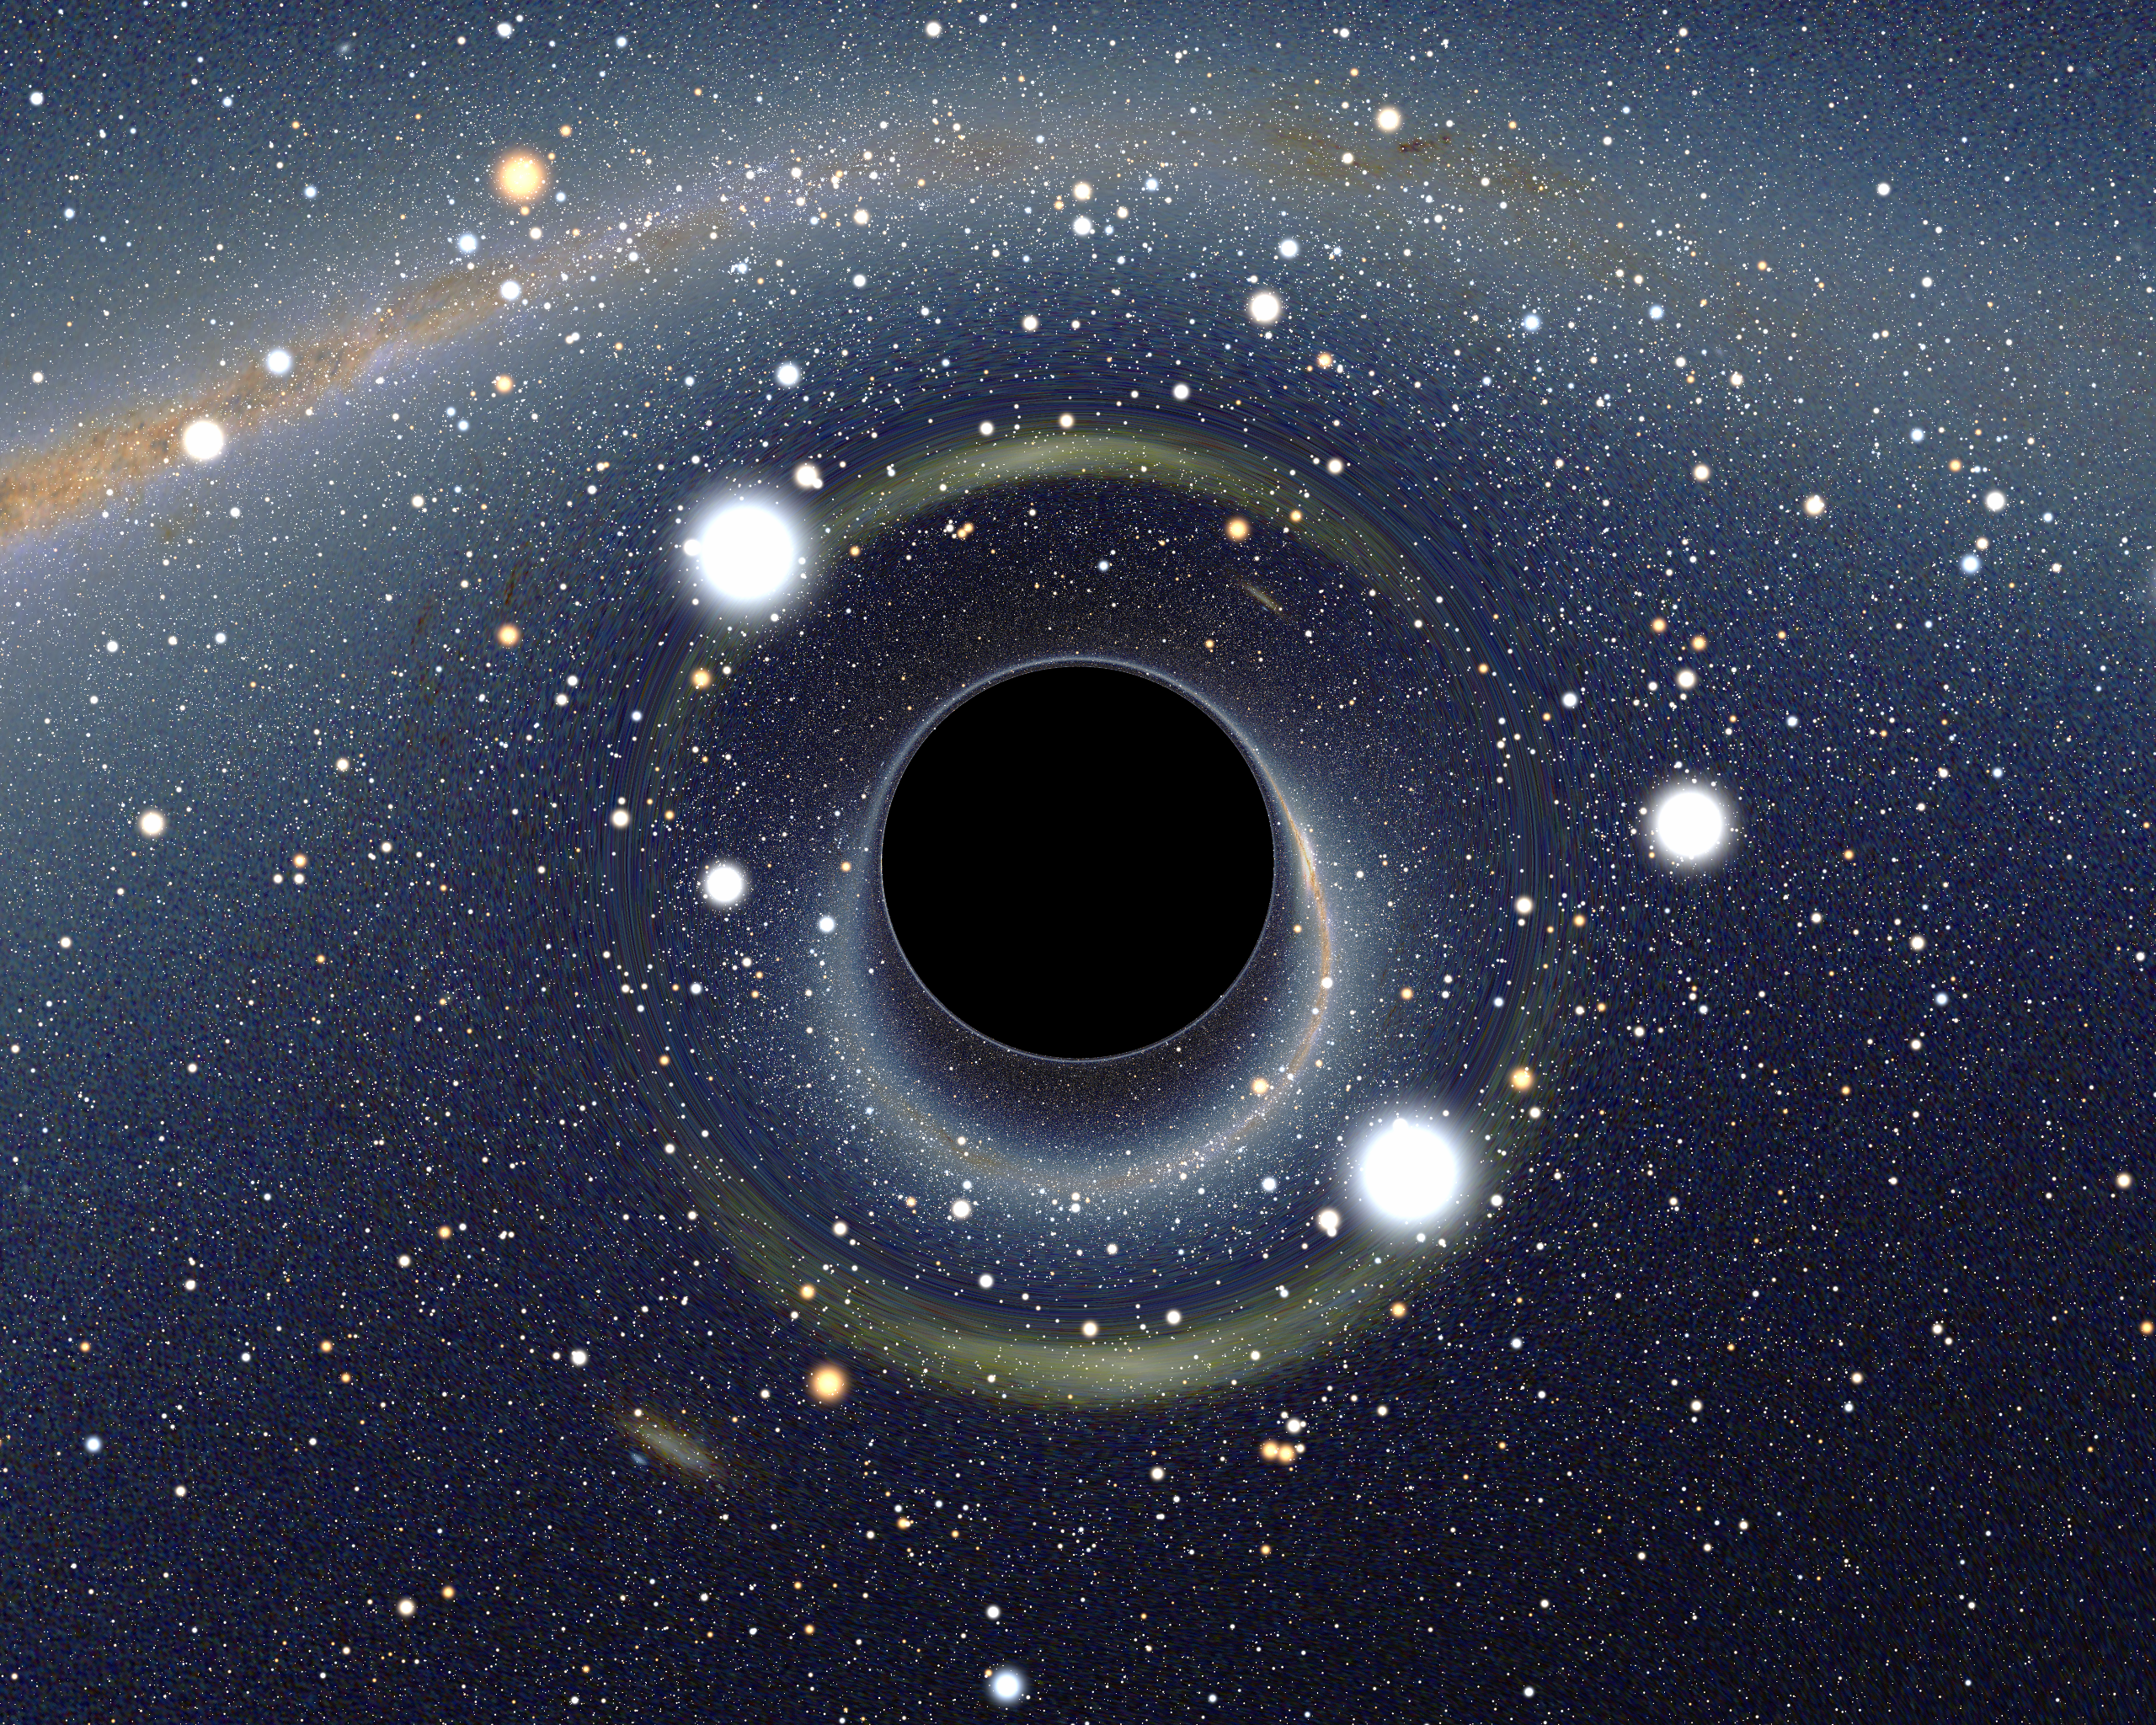
\includegraphics[width=9cm]{BH_LMC.png}%
\\
\textit{\footnotesize{Source: Wikipedia}}
\end{center}

\end{frame}



\addtocounter{page}{1}
\begin{frame}
\addtocounter{page}{-1}
\frametitle{That's it!}
%\framesubtitle{\hspace{5mm}Questions?}
\begin{center}
Thank you!\\
Questions?
\end{center}
\end{frame}



%\begin{frame}{Bibliography}
%\tiny
%\bibliography{bibliography}
%\end{frame}








\end{document}
